% flashcards-title: Packets and cards on aligned number lines
% flashcards-desc: Parallel number lines align two packets with six cards and five packets with an unknown card count.
\documentclass[dvisvgm,tikz,border=8pt]{standalone}\usetikzlibrary{arrows.meta,patterns}

\definecolor{qraNavy}{HTML}{17324D}
\definecolor{qraBlue}{HTML}{2B6CB0}
\definecolor{qraGold}{HTML}{B7791F}
\definecolor{qraPale}{HTML}{EAF2F8}
\definecolor{qraGray}{HTML}{5C6773}

\tikzset{
  qra axis/.style={draw=qraNavy, line width=1.2pt},
  qra tick/.style={draw=qraNavy, line width=1pt},
  qra guide/.style={draw=qraGray, densely dashed, line width=0.8pt},
  qra counter/.style={circle, draw=qraNavy, fill=qraPale, line width=0.9pt, minimum size=7mm, inner sep=0pt},
  qra label/.style={font=\sffamily\bfseries, text=qraNavy},
  qra small label/.style={font=\sffamily, text=qraNavy},
}

\begin{document}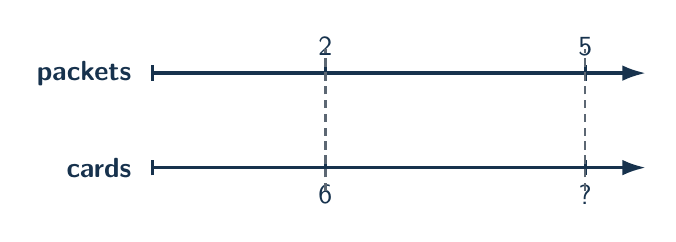
\begin{tikzpicture}[x=1.1cm,y=1cm]
\foreach \y/\lab in {1.2/{packets},0/{cards}}{\draw[qra axis,-{Latex[length=3mm,width=2mm]}](0,\y)--(5.7,\y);\foreach \x in {0,2,5}{\draw[qra tick](\x,\y-.1)--(\x,\y+.1);}\node[qra label,left=4pt]at(0,\y){\lab};}
\node[qra small label,above=3pt]at(2,1.2){2};\node[qra small label,above=3pt]at(5,1.2){5};\node[qra small label,below=3pt]at(2,0){6};\node[qra small label,below=3pt]at(5,0){?};\draw[qra guide](2,-.3)--(2,1.5);\draw[qra guide](5,-.3)--(5,1.5);
\end{tikzpicture}\end{document}
